\section{User Profile}

\begin{frame}[red]

\begin{itemize}
\item t-anonymity
\item POI
\item Protection types and schemes
\item Settings
\end{itemize}


\end{frame}


\subsection{t-anonymity \& POI} % Bookmark information, displayed in the progress tree
\begin{frame}[red] %hmm.. thought i could change colour here :S
\frametitle{t-anonymity}

\begin{definition}
Given $\mathbf{T}$, the set of trajectories, and a POI $p$.\\
Let $\Gamma \subseteq \mathbf{T}$, be the set of all trajectories which contains $p$.\\
Let $\Gamma^* \subseteq \Gamma$ and $\mathbf{TF}$ be some time frame, containing $p$, associated with $\Gamma^*$.\\
$\Gamma^*$ is said to satisfy t-anonymity with respect to $\mathbf{TF}$ iff:

\begin{enumerate}
	\item It contains at least $t-1$ other trajectories contained within $\mathbf{TF}$.

	\item The collection of timestamps entering $p$ ($\tau_{s}$) has at least one unique element. This has to hold for the collection of exiting timestamps ($\tau_{e}$) as well.
\end{enumerate}
\end{definition}

\end{frame}

\begin{frame}[red] %hmm.. thought i could change colour here :S
\frametitle{POI}

\begin{definition}
Let $\mathbf{P}$ be the collection of all POIs.\\
Each POI $p \in \mathbf{P}$ is a tuple $(p_{cover}, d_s, d_t)$ where $p_{cover}$ is the set of edges $e \in \mathbf{E}$ which the POI covers and \\
$d_s, d_t \in \mathbb{N}$ is the spatial and temporal sensitivity respectively.
\end{definition}

\end{frame}

\subsection{Protection Schemes \& Types} % Bookmark information, displayed in the progress tree
\begin{frame}[red] %hmm.. thought i could change colour here :S
\frametitle{Protection Schemes \& Types}

Protection Types
\begin{enumerate}
	\item Area containing POI (spatial)
	\item k-anonymity (spatial)
	\item Timeframe containing the POI and its visitation time. (temporal)
	\item t-anonymity (temporal)
\end{enumerate}

\vspace{1em}

Protection Schemes
\begin{itemize}
	\item AS - Always Sensitive.
	\item ASTI - Always Sensitive within a time interval.
	\item RS - Rarely Sensitive.
\end{itemize}

\end{frame}

% 
% \begin{frame}[red]
% 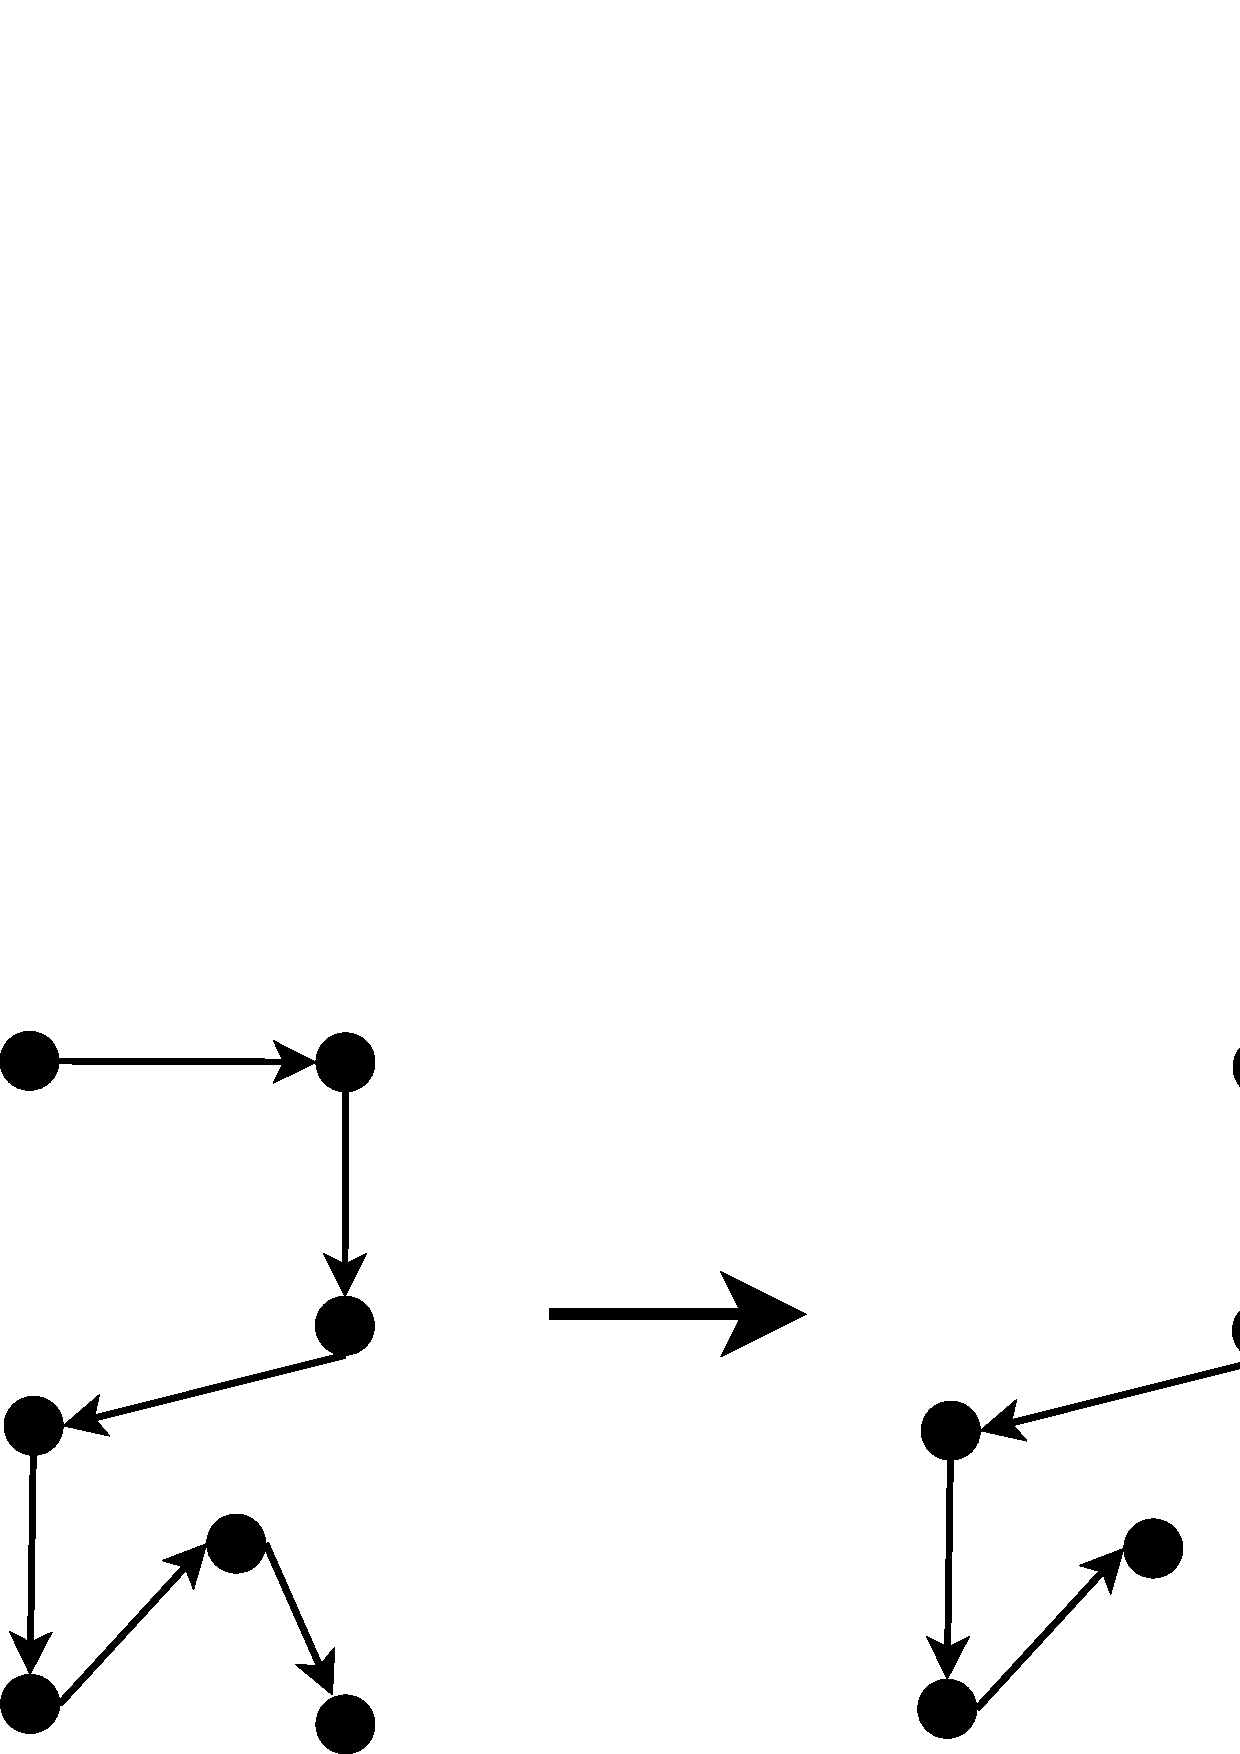
\includegraphics[page=1,scale=0.5]{images/traDel.pdf}
% \end{frame}


\begin{frame}[red]
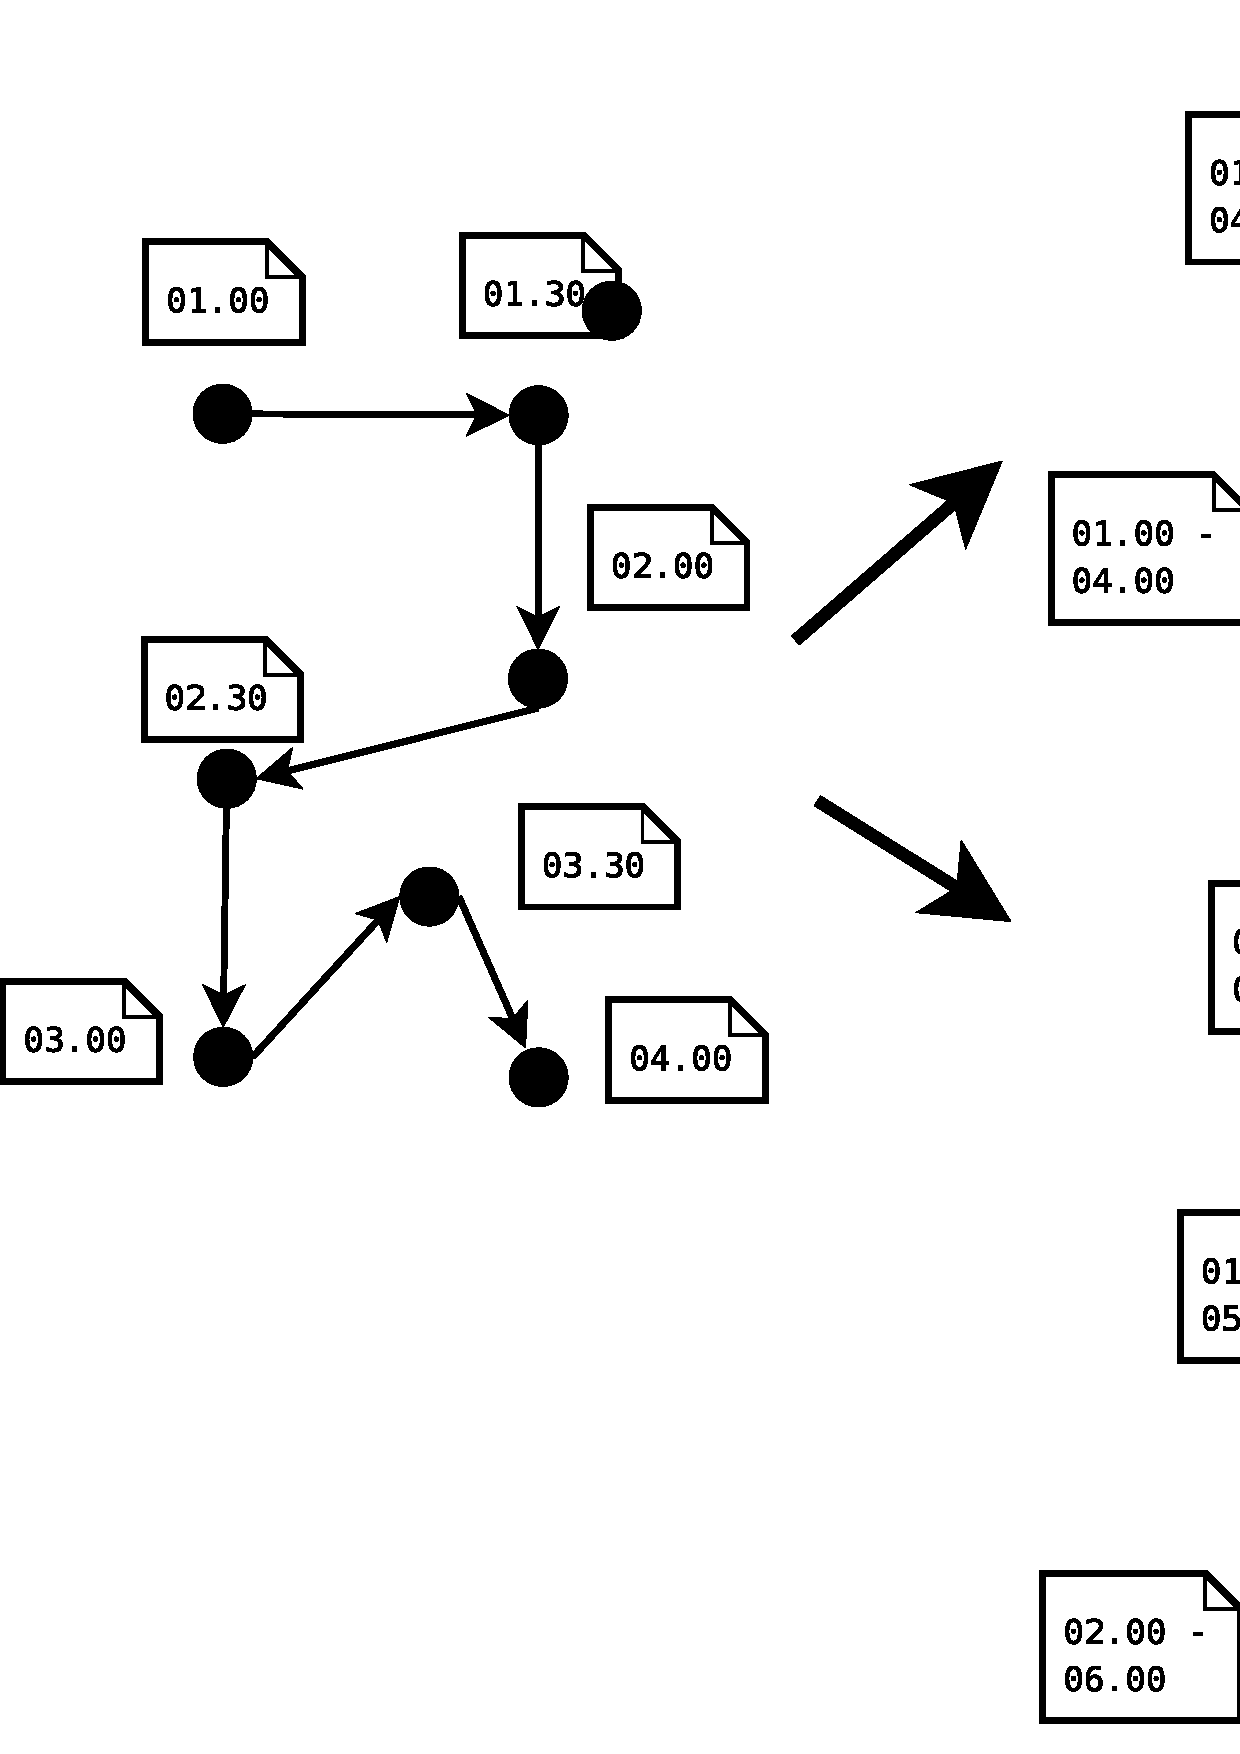
\includegraphics[page=1,scale=0.22]{images/traTime.pdf}
\end{frame}



\begin{frame}[red] %hmm.. thought i could change colour here :S
\frametitle{POI Types}

\begin{table}
%\begin{tabular*}{0.8\columnwidth}{|p{0.2\columnwidth}|l|p{0.25\columnwidth}|}
\begin{tabular}{|l|l|l|}
\hline
POI type 		& Protection type & Scheme \\\hline
Hospital		& 1,3 & AS \\\hline
Private home (house)	& 1-3 & ASTI, RS \\\hline
Neighborhood		& 1,3 & ASTI, RS  \\\hline
City part		& 1,3,4 & ASTI, RS  \\\hline
City			& 1,3 & ASTI, RS  \\\hline
Route w/o endpoints	& 1,3 & AS, ASTI, RS  \\\hline
Route w. endpoints	& 1-4 & AS, ASTI, RS  \\\hline
%\end{tabular*}
\end{tabular}
\end{table}

\begin{enumerate}
	\item Area containing POI
	\item k-anonymity
	\item Timeframe containing the POI and its visitation time.
	\item t-anonymity
\end{enumerate}

\end{frame}




\subsection{Settings} % Bookmark information, displayed in the progress tree


\begin{frame}[red] %hmm.. thought i could change colour here :S
\frametitle{Settings}

Users Can
\begin{itemize}
\item Set Temporal sensitivity
\item Set Spatial sensitivity
\item Define which edges in a road map that a POI covers
\item Set the scheme to be used with a POI
\item Can have multiple profiles.
\end{itemize}

\end{frame}

